\newpage

\section{Programmverwendung}


\subsection{Verwendung der graphischen Ansicht}

Nach dem Programmstart befindet sich der Benutzer üblicherweise in der graphischen Ansicht.

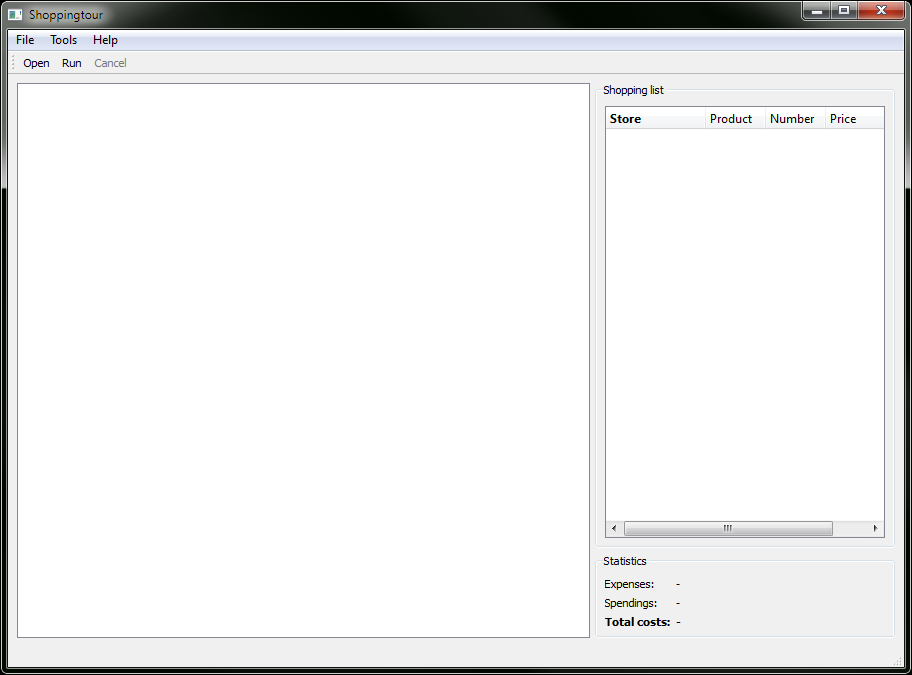
\includegraphics[width=1\textwidth]{resourcen/walkthrough/0-default-view.png}

\newpage

Der Benutzer öffnet nun eine Problemdefinition, in dem er den \emph{Open}-Button in der Toolbar, oder wahlweise den gleichnamigen Menüpunkt im File-Menü, verwendet. Hierbei hat er die Wahl zwischen den beiden implementierten Algorithmen.

In der folgenden Ansicht wählt der Benutzer die Problembeschreibungsdateien über den \emph{Select}-Button oder durch manuelle Eingabe in das Textfeld aus.

Für die Verwendung von Clingo zur Problemlösung muss der Pfad zur ausführbaren Programmdatei angegeben werden. In der \emph{Windows One-Click Distribution} befinden sich diese im dist/clingo-Ordner; Windows-Benutzer müssen hier also den Pfad zur \texttt{w32clingo.exe}-Datei, also beispielsweise \texttt{dist/clingo/w32clingo.exe}, angeben. Der Pfad kann hierbei absolut oder relativ zum aktuellen Arbeitsverzeichnis angegeben werden.

Alternativ kann der Benutzer den genetischen Algorithmus wählen. Hierbei kann er die Eckdaten des Algorithmenverhaltens bestimmen. Die Beschreibung der Buttonfunktionen kann über den \emph{Help}-Button erfahren werden.

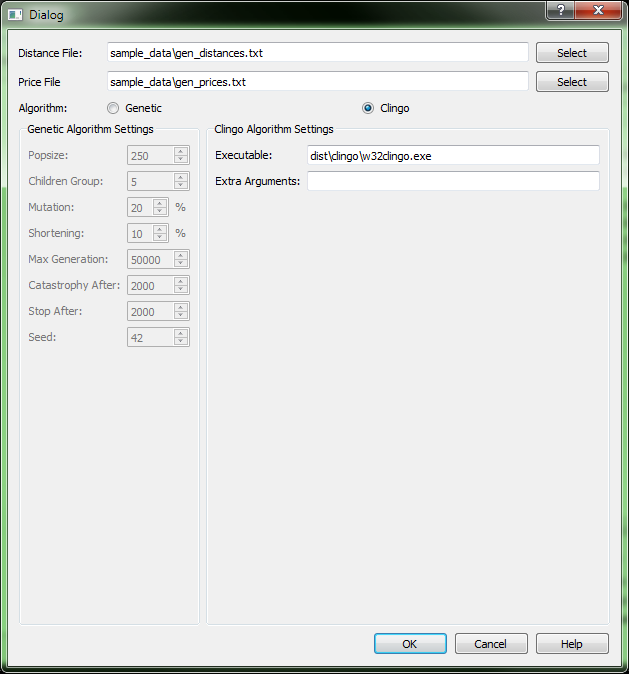
\includegraphics[width=0.48\textwidth]{resourcen/walkthrough/1a-open-clingo.png} 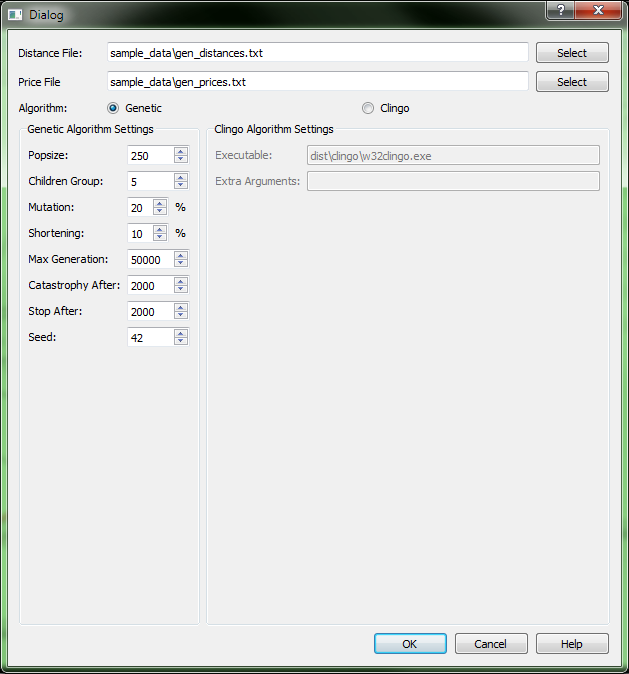
\includegraphics[width=0.48\textwidth]{resourcen/walkthrough/1b-open-genetic.png}

\newpage

Der Benutzer sieht nun eine graphische Darstellung des Problembereiches. Er kann per Klicken und Ziehen die einzelnen Knoten des Graphen verschieben (optional kann er die Funktion der elastischen Knoten im ''Tools''-Menü aktivieren).

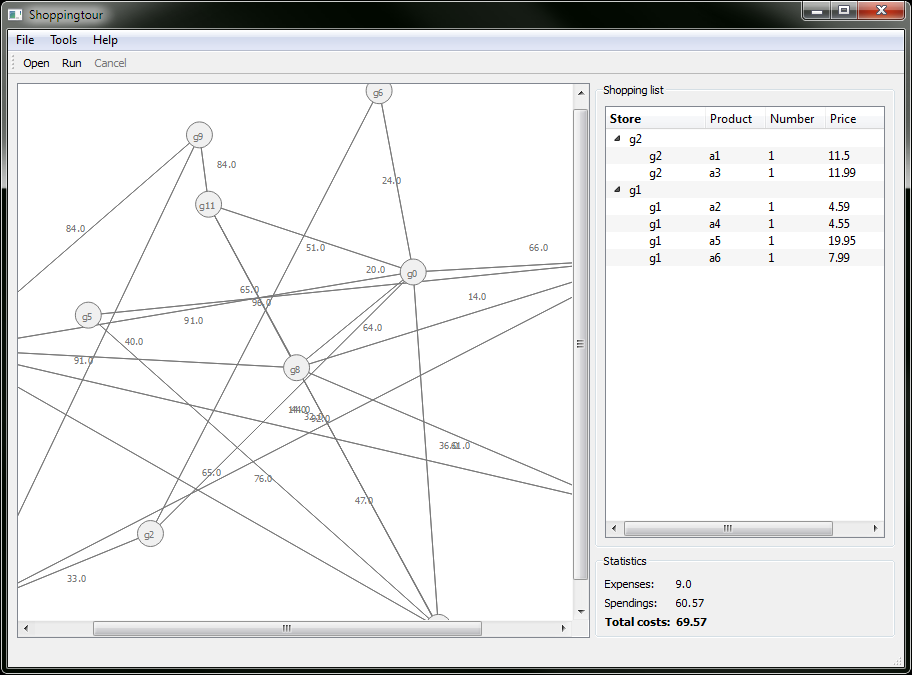
\includegraphics[width=1\textwidth]{resourcen/walkthrough/2-opened-clingo.png}

\newpage

Um die Berechnung zu starten, klickt der Benutzer auf den \emph{Run}-Button in der Toolbar. Während des Algorithmen-Durchlaufs wird ihm der aktuelle Programmzustand, also die aktuell berechnete (Teil-) Lösung, graphisch und in Listenform dargestellt.

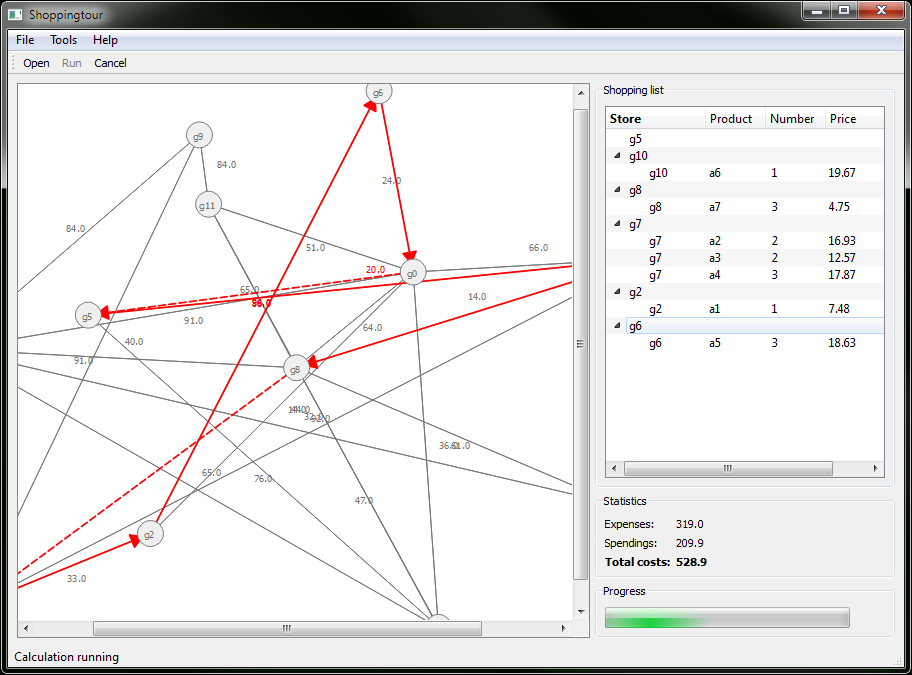
\includegraphics[width=1\textwidth]{resourcen/walkthrough/3-running-clingo.png}

\newpage

Der Benutzer kann den Berechnungsvorgang selbstverständlich auch abbrechen. Hierzu wählt er entweder in der Toolbar die \emph{Cancel}-Option oder alternativ die gleichnamige im Tools-Menü.

In der Endansicht wird der Benutzer über die beste gefundene Lösung informiert. Dies geschieht auch hier einerseits in graphischer Form und andererseits in Listenform. Die Listenform wird als \emph{Shopping list} bezeichnet und beschreibt, in welcher Reihenfolge welche Geschäfte besucht werden sollen (erste Baumebene) und welche Gegenstände in welcher Anzahl dort gekauft werden sollen (zweite Baumebene).

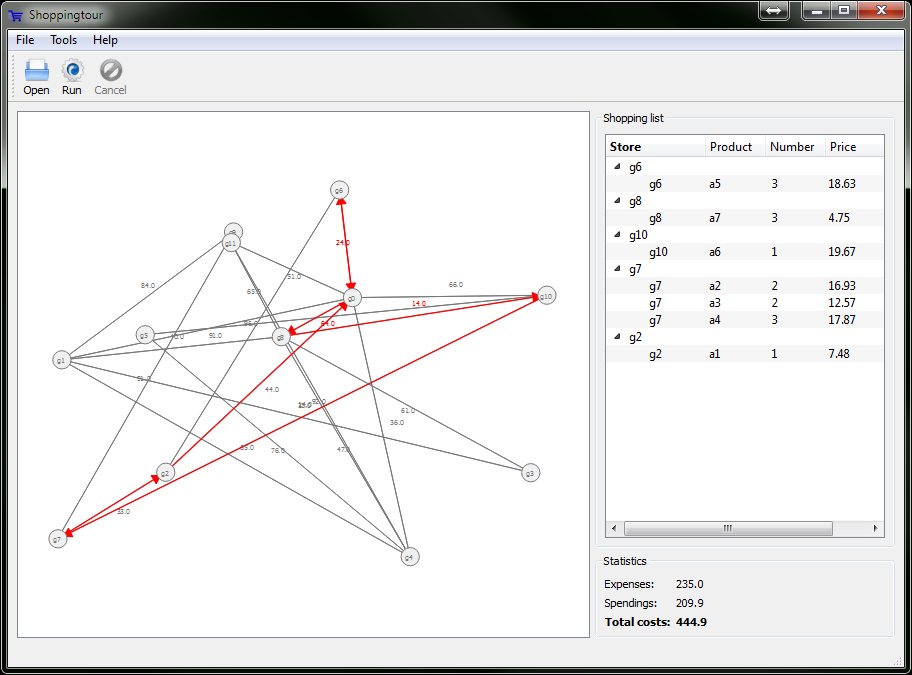
\includegraphics[width=1\textwidth]{resourcen/walkthrough/4-finished-clingo.png}

\newpage